\documentclass{lni}

\IfFileExists{latin1.sty}{\usepackage{latin1}}{\usepackage{isolatin1}}

\usepackage{graphicx}

\author{Nikolaus Moll\\\\abc@def.de}
\title{Modellierung und Generierung von Test-Daten f�r Datenbank-basierte Anwendungen}
\begin{document}
\maketitle

\begin{abstract}
Softwaretests haben sich als Teil der Qualit�tssicherung von Softwareprojekten etabliert.
F�r Tester ist die Modellierung von Testdaten f�r Datenbank-basierte Anwendungen allerdings
nicht immer einfach. Die Daten k�nnen aufgrund von Beziehungen von Datens�tzen schnell
un�bersichtlich und komplex werden. Wegen der Komplexit�t versuchen Tester, mehrere Tests
mit denselben Daten durchzuf�hren.

In dieser Masterarbeit werden eine neue Modellierungssprache f�r Testdaten f�r
Datenbank-basierte Anwendungen und ein Algorithmus zur Generierung von Testdaten 
vorgestellt. Die Sprache erlaubt eine �bersichtliche Beschreibung von Daten und
von Beziehungen zwischen Datens�tzen. Der Algorithmus zur Generierung erzeugt
Daten anhand der Beziehungstypen im Datenbank-Modell. Der Algorithmus versucht
viele Grenzf�lle zu erzeugen, so dass die Daten in m�glichst vielen Tests verwendet
werden k�nnen.
\textit{Apache License 2.0}.

\end{abstract}


\section{Einleitung und Motivation}

Softwaretests sind ein wichtiger Baustein f�r die Qualit�tssicherung von modernen Softwareprojekten.
F�r Tests werden Testdaten spezifiziert. Auf deren Basis wird das Verhalten der Software gepr�ft.
Bei Datenbank-basierten Anwendungen werden Testdaten in der Regel sehr umfangreich und komplex.

Die Komplexit�t ergibt sich aus der Beschreibung von Beziehungen zwischen den einzelnen
Datens�tzen. Besonders bei Systemen mit komplexen Datenbank-Schemata kann ein
Testdaten-Modell schnell un�bersichtlich werden.

F�r den Tester sind un�bersichtliche Testdaten aus verschiedenen Gr�nden ein Problem.
Einerseits machen sie die Pflege fehleranf�llig. Andererseits ist es schwer,
die modellierten Daten zu erfassen und zu verstehen. Tester w�nschen deshalb h�ufig Daten,
die f�r mehrere Tests nutzbar sind. Dadurch reicht es aus, nur ein oder zumindest
wenige Daten-Modelle zu verstehen und zu pflegen.

Die im Rahmen einer Master Thesis [Quelle] entwickelte Modellierungssprache f�r Testdaten erlaubt
eine �bersichtliche Modellierung von Testdaten. Sie ist einfach zu nutzen und integriert sich
in g�ngige Entwicklungsumgebungen.

Dar�ber hinaus wurde ein Algorithmus f�r die Generierung von Testdaten konzipiert. Das Ziel des
Generators ist es, mit wenigen Datens�tzen viele Grenzf�lle bei Beziehungen abzudecken.


\section{Die Modellierungssprache}

	\subsection{Sprach-Definition}

	\subsection{Anwendung der Sprache}
	
	- Definieren eines Datenbank-Modells
	
	- Generieren der DSL
	
	- Unit-Test-Beispiel
	

	\subsection{Implementierung und Evaluation}
	
	- Implementiert auf Java-Basis mit Groovy
	
	- Apache 2 Lizenz
	
	- http://github.com/seitenbau/stu
	
	- Implementierungsdetails in Thesis
	
	- Einsatz in Beispielen und realen Projekten gepr�ft
	


\section{Der Test-Daten-Generator}
Idee hinter dem Algorithmus

	\subsection{Beschreibung des Algorithmus}

	\begin{figure}[htb]
		\begin{center}
			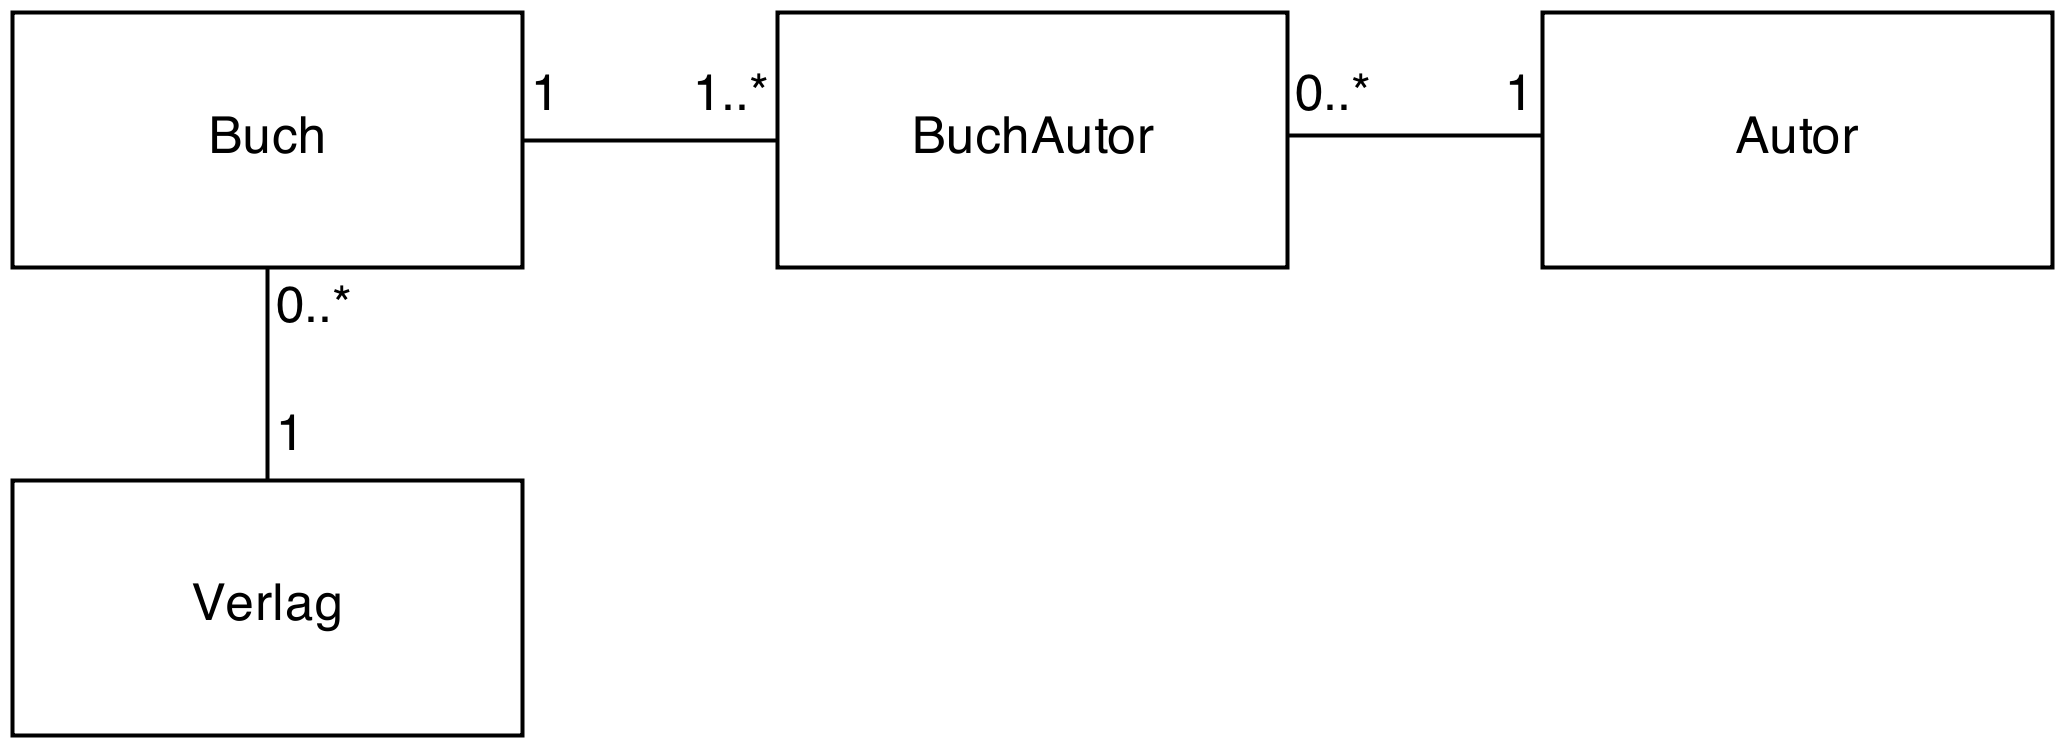
\includegraphics[width=8cm]{images/database.png}
			\caption{\label{database}Datenbank-Diagramm}
		\end{center}
	\end{figure}
	
	\subsubsection{

	

	\subsection{Implementierung und Evaluation}

\section{Fazit}

\bibliography{bibliography}

\end{document}



